\documentclass[]{article}

\usepackage{amsmath}
\usepackage{amssymb}
\usepackage{graphicx}
\usepackage[utf8]{inputenc} 
\usepackage{subcaption}
\usepackage{caption}
\usepackage{hyperref} 
%opening
\title{}
\author{}

\begin{document}

\maketitle

\begin{abstract}
\end{abstract}


\section{Weighted operator tests}

\subsecion{Convergence of the weights}
We fix $N=40$, lift macroscopic steady states with the weighted operator $\mathcal{L}_W$ and plot the weighted distribution as a function of the number of realizations $M$.

\begin{figure}
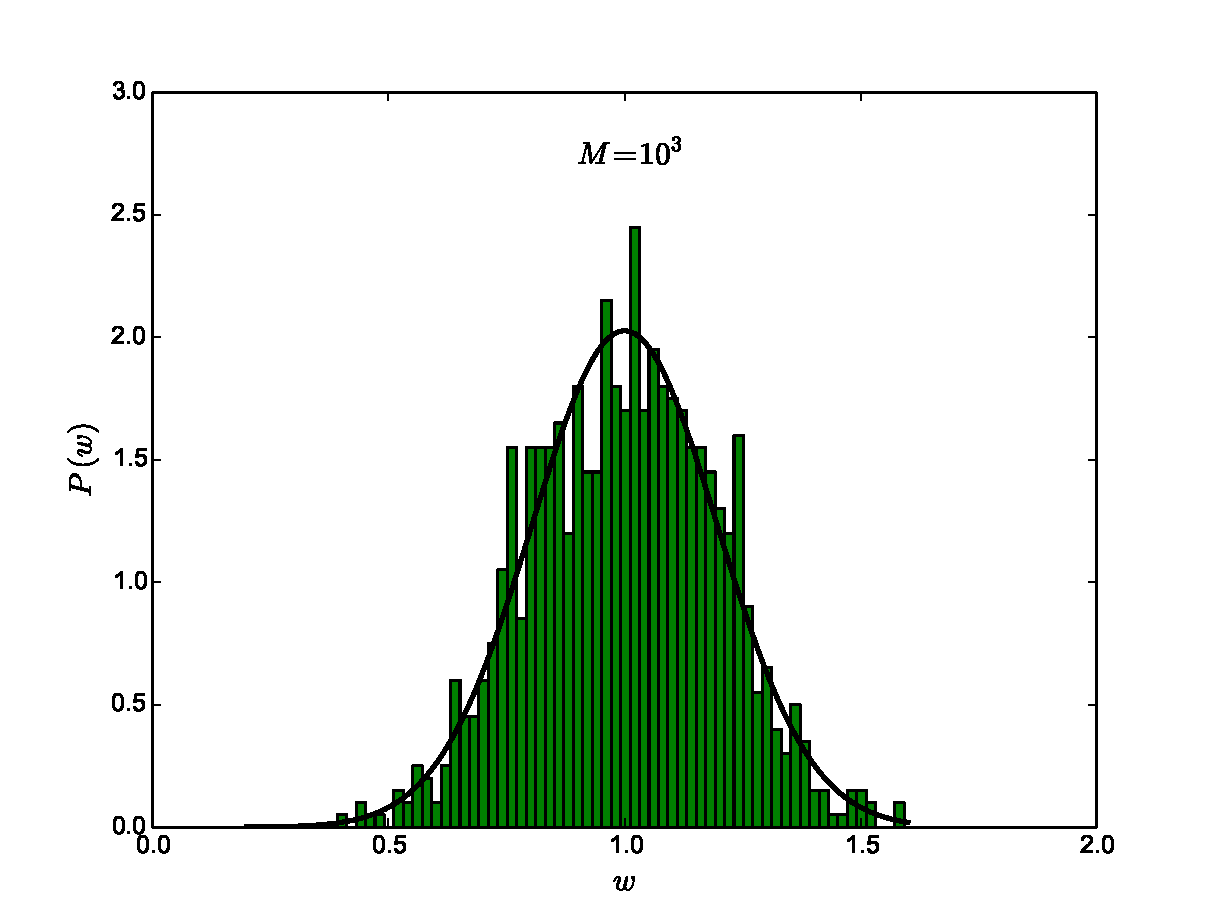
\includegraphics[width=0.9\textwidth]{weights_E1_M1000.pdf}
\caption{We observe that the weight distribution for mixed states is well approximated by a Gaussian}
\label{fig:hist_weights}
\end{figure}

\begin{figure}
\includegraphics[width=0.9\textwidth]{weights_E1_M400to8000.pdf}
\caption{Distribution of weights as a function of $M$
\label{fig:hist_weights}
\end{figure}

\subsection{Convergence of the Jacobian-vector product}



\begin{figure}
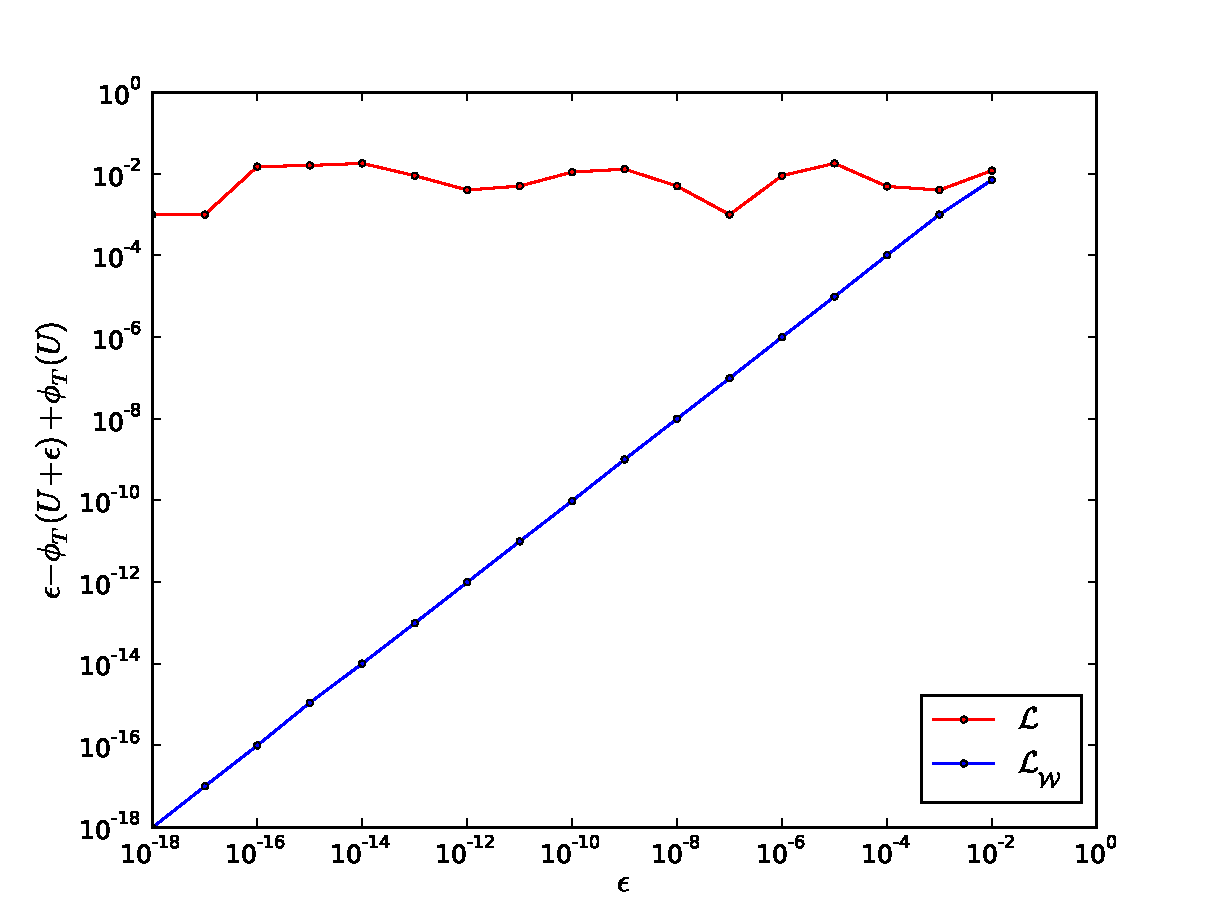
\includegraphics[width=0.9\textwidth]{epsilon_dependence_M1000_N40_1dim.pdf}
\caption{For the red plot, the coarse time-stepper was calculated without weights and for two independent function evaluations. For the blue plot we used weighted operators calculated with the same realizations, microscopic parameters and random time paths. For both simulations we used $N=40$, $M=1000$ and a time horizon of 5 steps in the coarse time steppers. We only collected statistics of one particle.}
\label{fig:epsilon}
\end{figure}

\end{document}
